% Title: Report LaTex File: Hardware Development
% Auther: DC Eksteen
% Student Number: 22623906
% Contact: 22623906@sun.ac.za
% Date: 2022/09/14
% Version: 2.0

\chapter{Hardware Development}
% Section overview: Hardware development.

For the project, hardware was developed with the aim of achieving the objectives shown in \ref{tab:devgoals} below:

\begin{table}[H]
	\color{red} % Comment if section finalized
	\renewcommand{\arraystretch}{1.2}
	\centering
	\caption{Objectives of Hardware Development}
	\begin{tabularx}{\textwidth}{p{2cm} >{\raggedright}p{5cm} >{\raggedright\arraybackslash}X}
		\toprule
		Hardware Design Outcome & Description          & Required Outcome            \\
		\midrule
		HDO 1            & Eddy Current Brake      & Design for adaptable length \\
		HDO 2            & Speed Sensors & Adequate Braking Force      \\
		HDO 3            & Frame and Shafts            & Description                 \\
		HDO 4            & Outcome 4            & Description                 \\
		\bottomrule
	\end{tabularx}
	\label{tab:devgoals}
\end{table}

\newpage

\section{Expected Operating Conditions}

Roller trainers require the cyclist to be travelling at some speed for stability. Thus, the expected operating range of a cyclist on the trainer will typically range between \SI{10}{\kilo\meter\per\hour} and \SI{50}{\kilo\meter\per\hour}. For the design, a maximum high speed of \SI{60}{\kilo\meter\per\hour} was considered. The corresponding drum speeds are shown in Figure \ref{fig:speedCalc} below.

\begin{figure}[H]
	\begin{center}
		\includegraphics[width=0.5\textwidth]{SpeedCalculations.jpg}
		\caption{Rotational Speed of Roller Size Comparison}
		\label{fig:speedCalc}
	\end{center}
\end{figure}

For the Eddy Current brake, as discussed in Section \ref{sec:Eddy}, higher speeds will result in higher braking force and thus a larger available resistance range. On the other hand, higher speeds will also increase the free-rolling resistance of the trainer, and allow for less range at higher speeds. Thus, \SI{90}{\milli\meter} drums were selected as a good compromise, and were selected for the model.\\

Typical cyclists average between 75 and \SI{100}{\watt}, and pro cyclists can reach up to \SI{400}{\watt}, during a 1 hour workout. 

\newpage

\section{Eddy Current Brake Design}
\label{sec:Eddy}

\begin{figure}[H]
	\begin{center}
		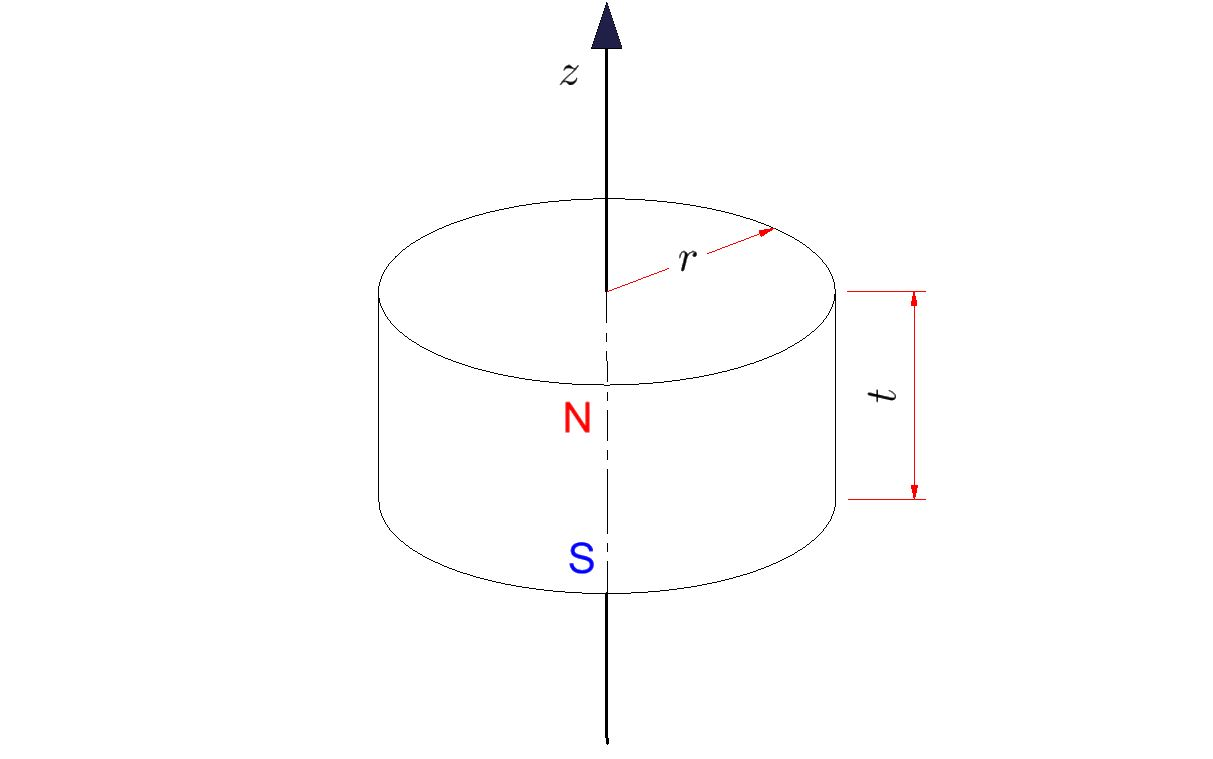
\includegraphics[width=0.5\textwidth]{magnetBr.jpg}
		\caption{Magnetic Flux Density of Disc Magnet}
		\citep[Addapted from][]{Supermagnete:2010}
		\label{fig:B0}
	\end{center}
\end{figure}

\begin{equation}
	\acs{B} = \frac{\acs{Br}}{2} (\frac{t+ z}{\sqrt{r^2 + {t + z}^2}} - \frac{z}{r^2 + z^2})
	\label{eq:B}
\end{equation}

\begin{figure}[H]
	\centering
	\begin{subfigure}[b]{.475\textwidth}
		\centering
		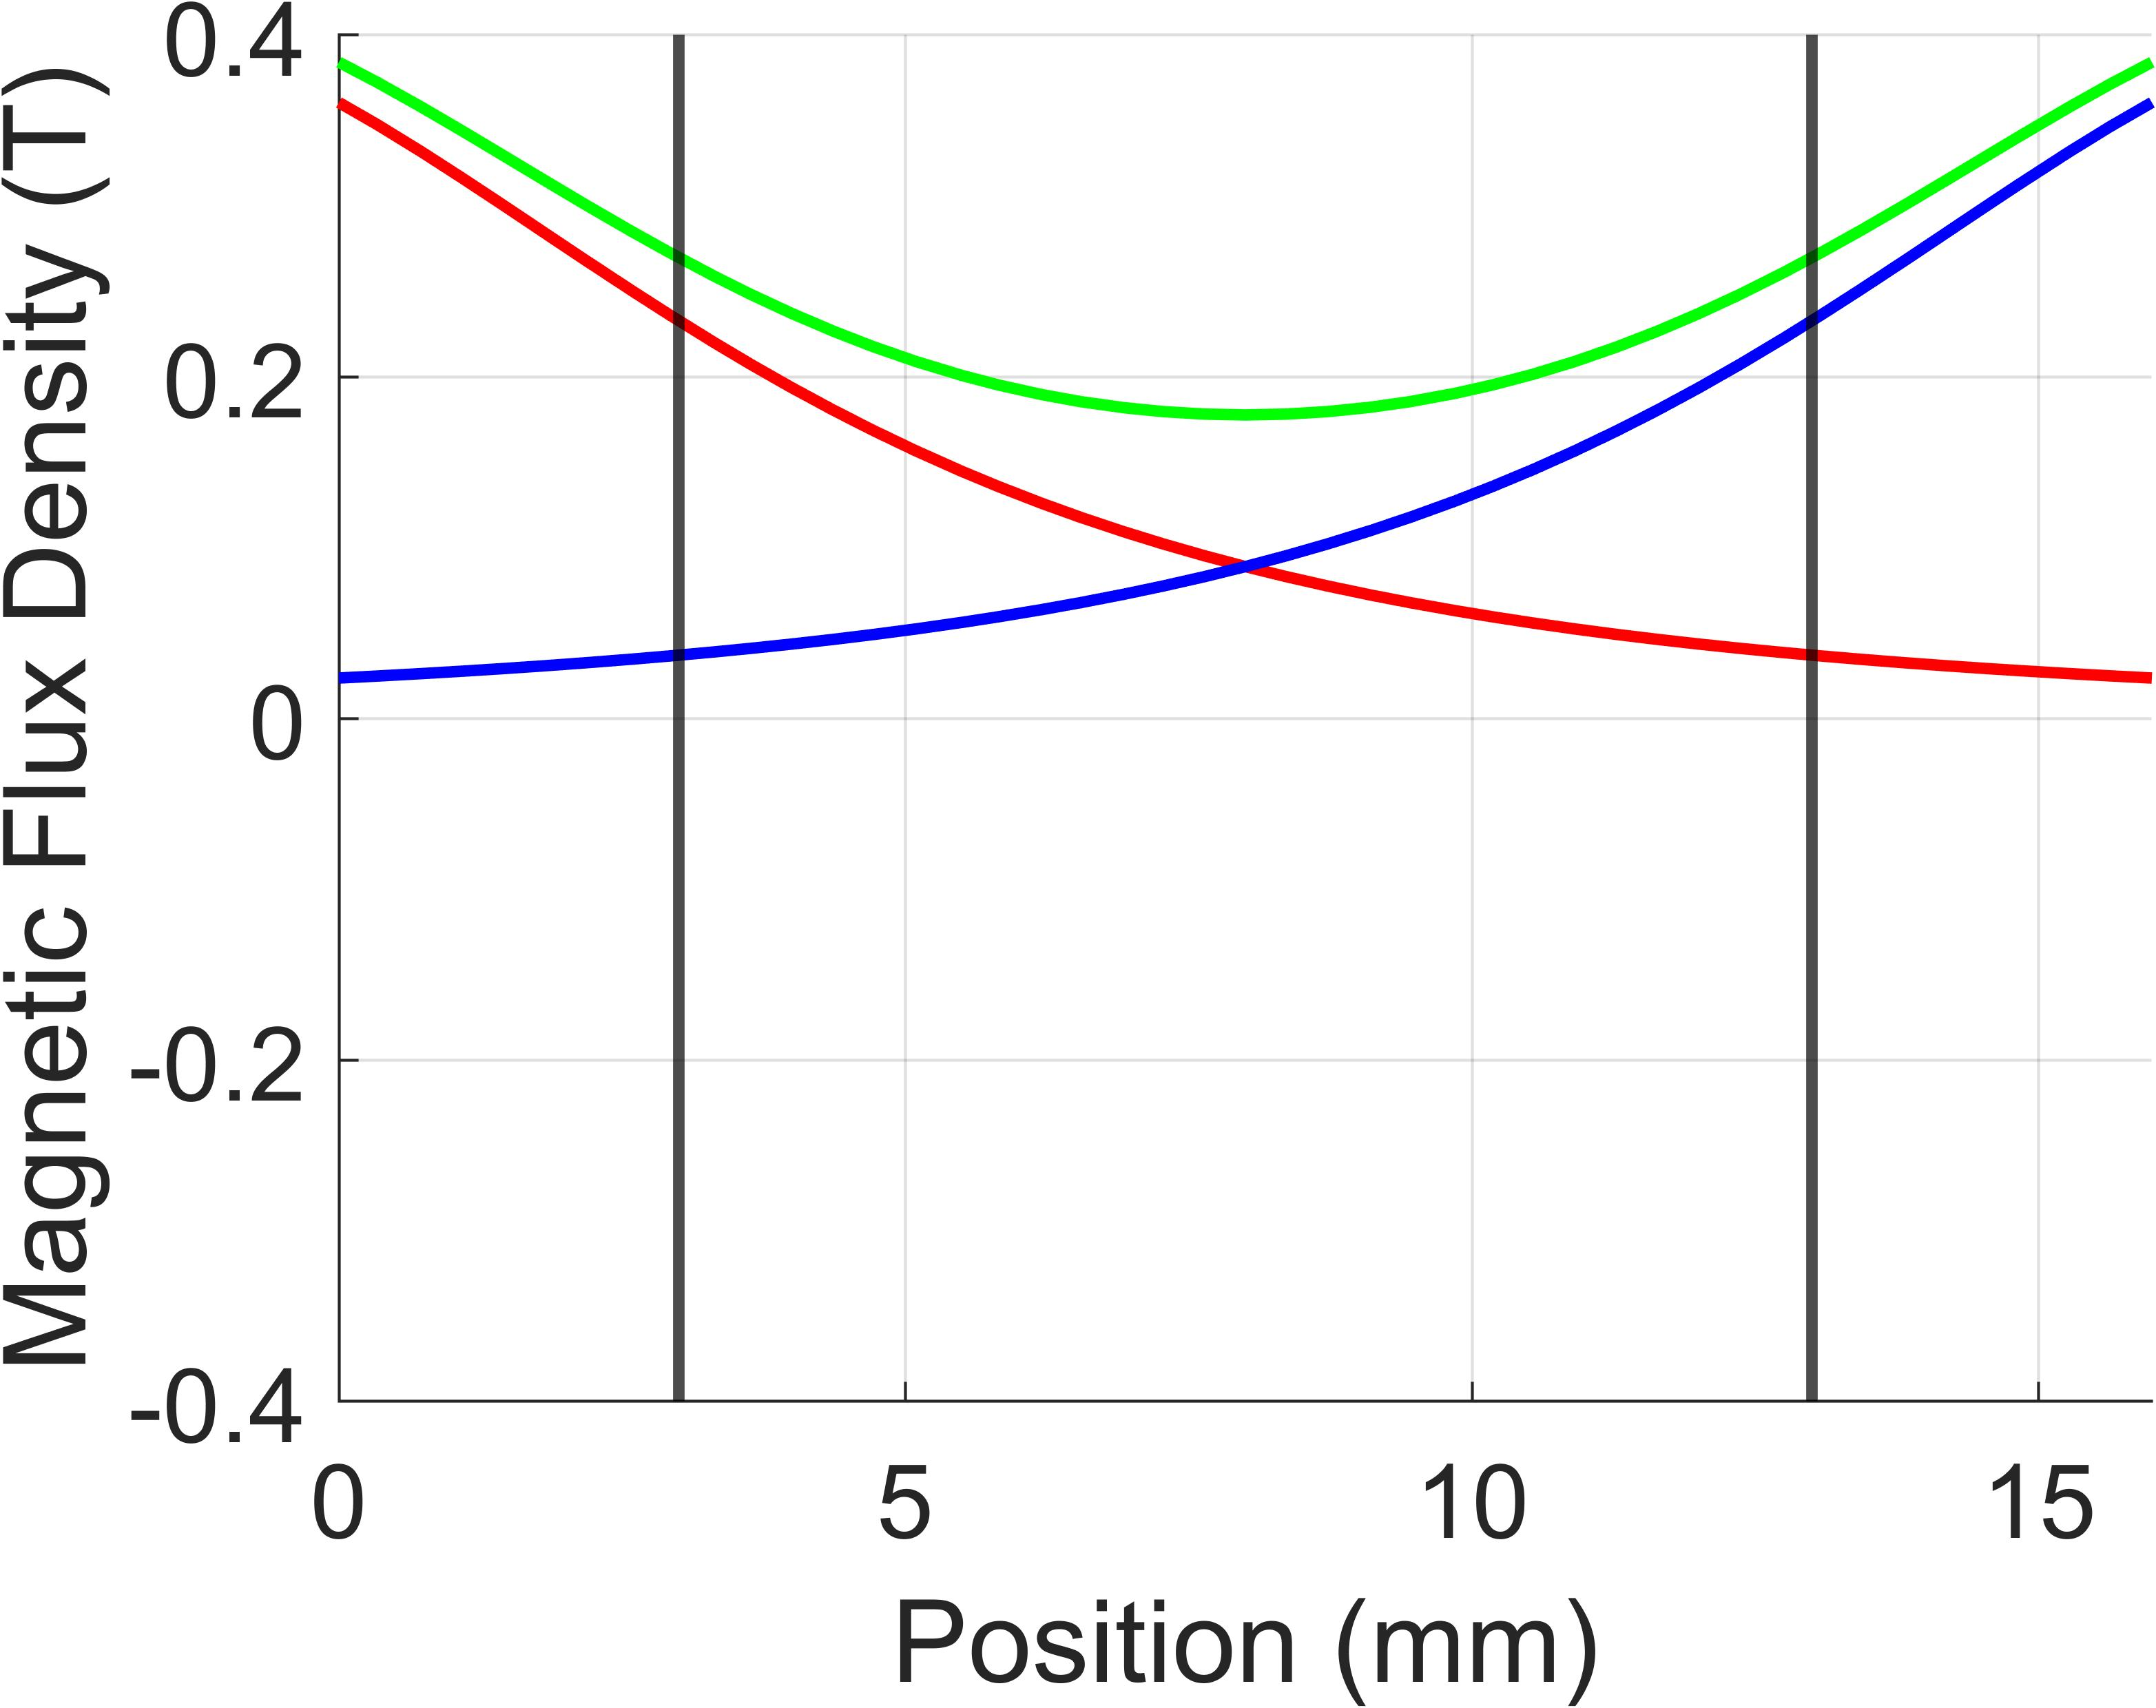
\includegraphics[width=.9\linewidth]{FluxZeroDeg.jpg}
		\caption{\SI{0}{\degree} Phase}
		\label{fig:Flux0}
	\end{subfigure}
	\hfill
	\begin{subfigure}[b]{.475\textwidth}
		\centering
		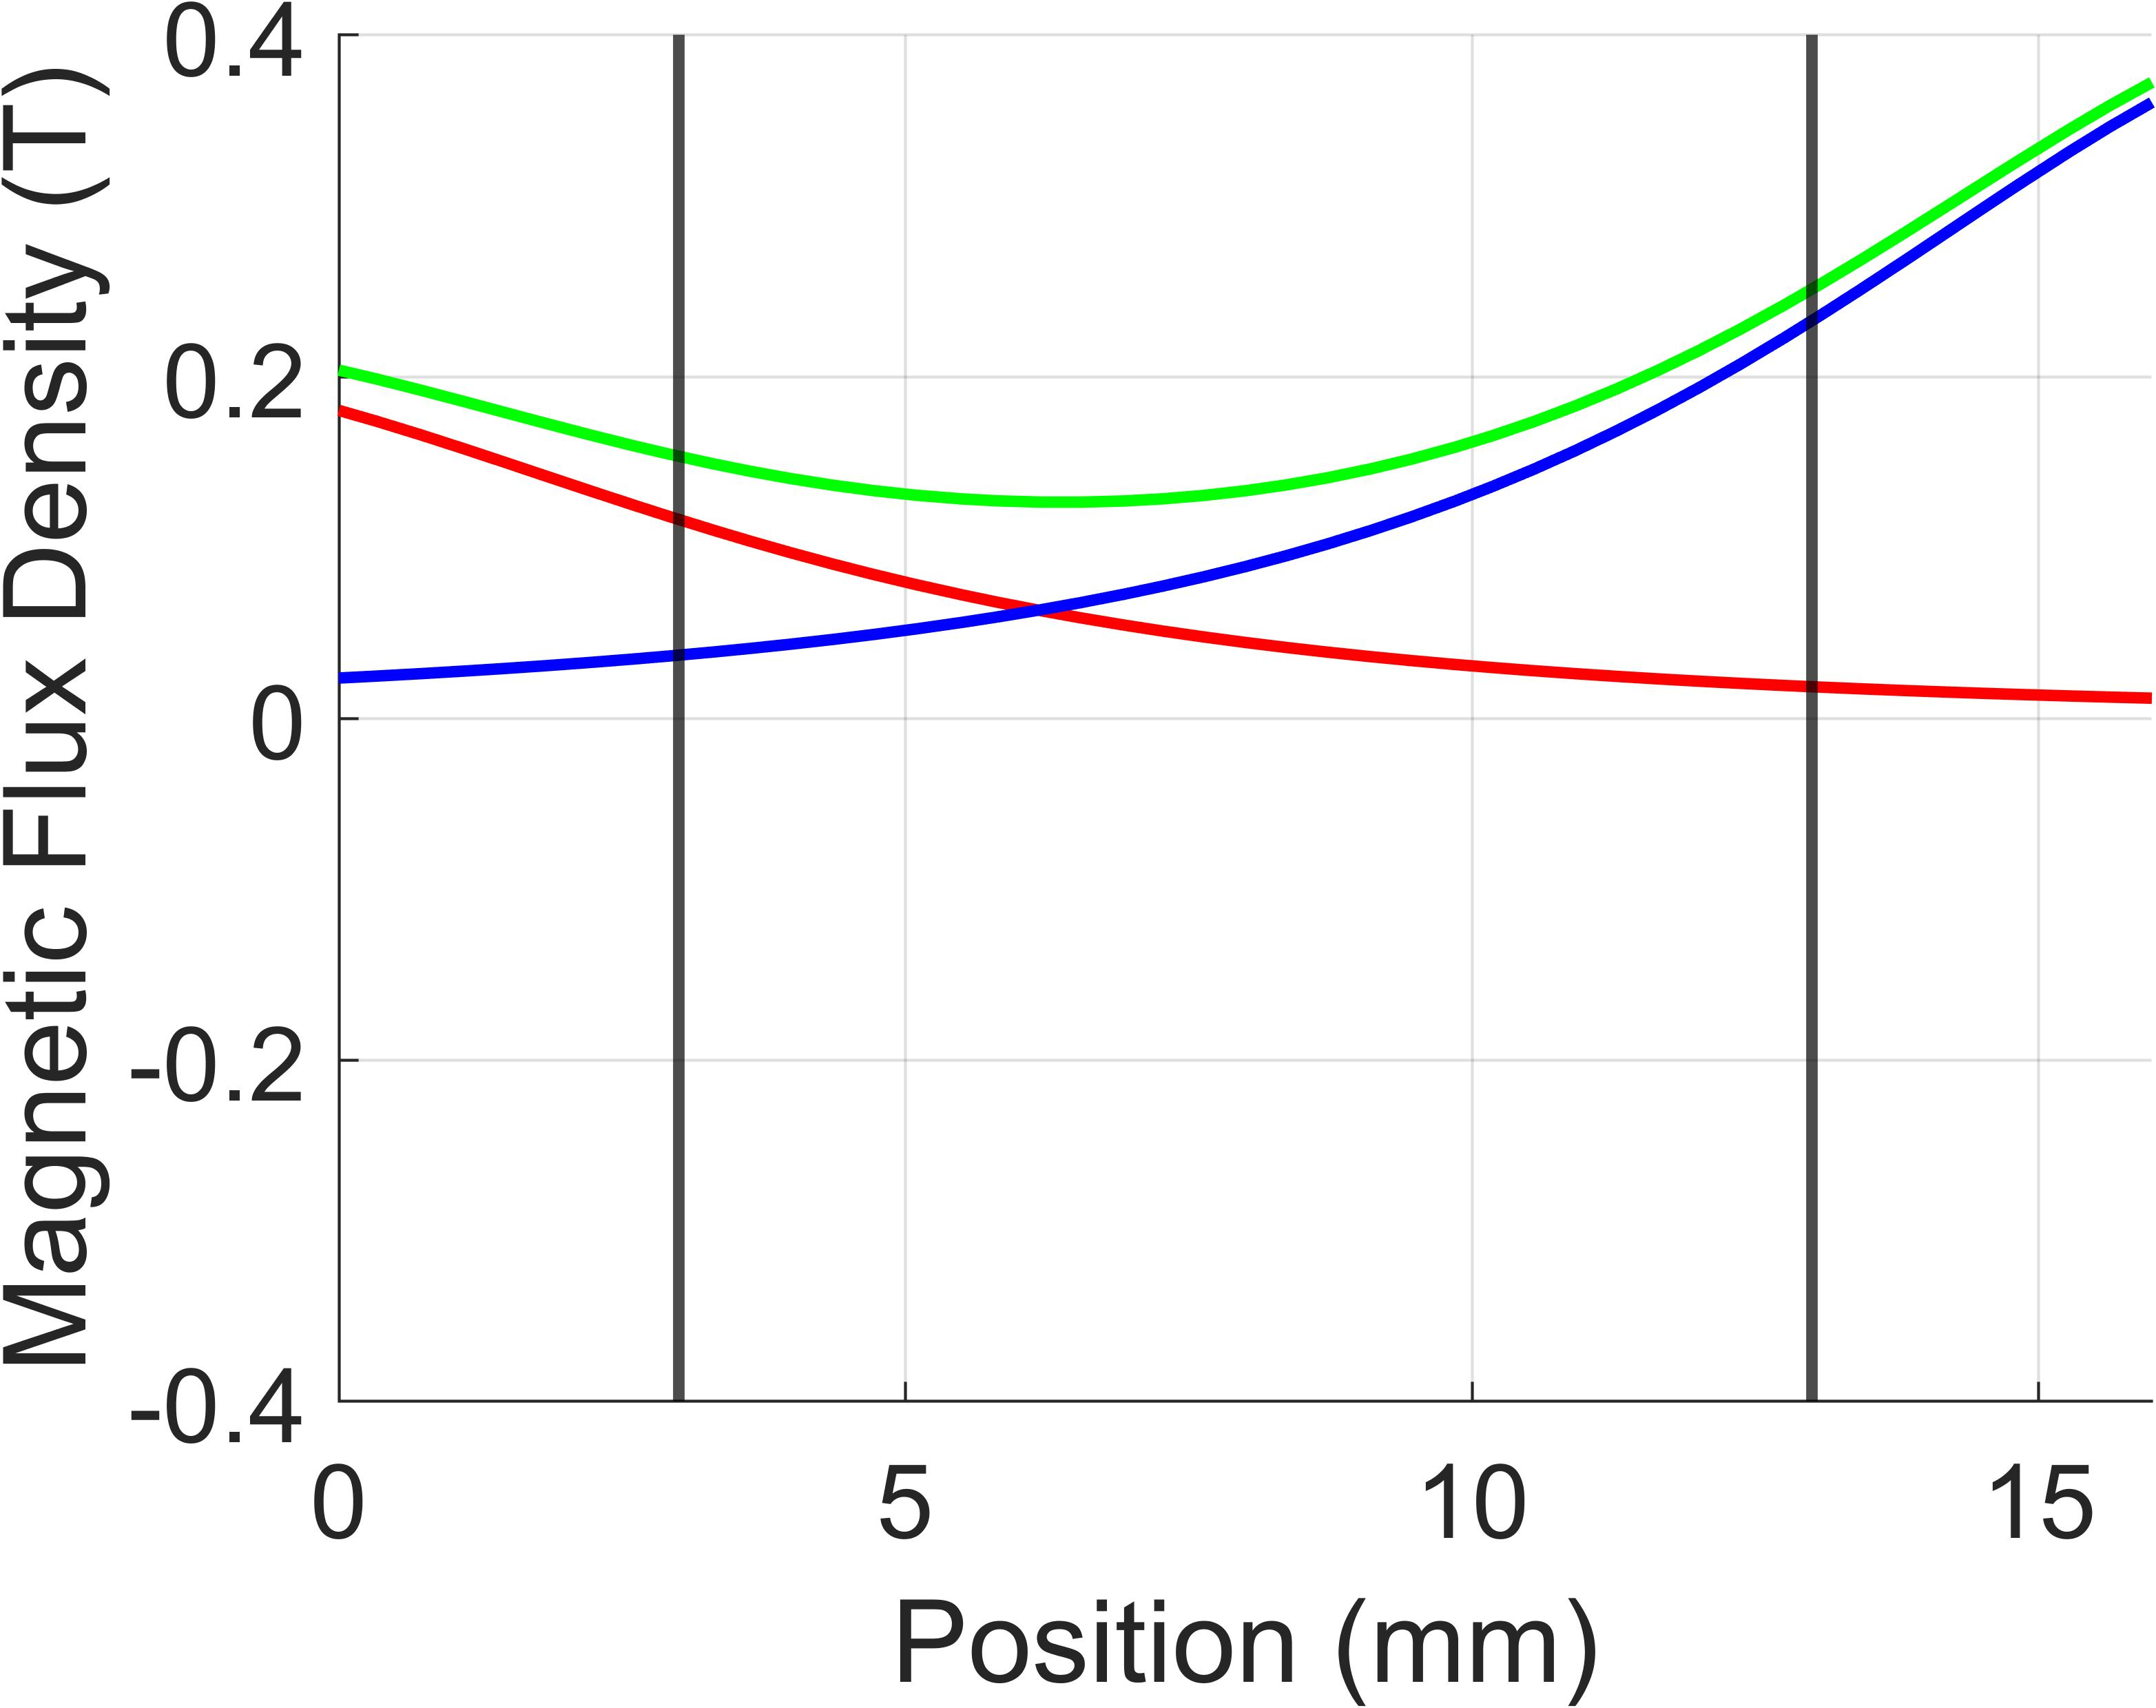
\includegraphics[width=.9\linewidth]{FluxSixtyDeg.jpg}
		\caption{\SI{60}{\degree} Phase}
		\label{fig:Flux60}
	\end{subfigure}
	\vskip\baselineskip
	\begin{subfigure}[b]{.475\textwidth}
		\centering
		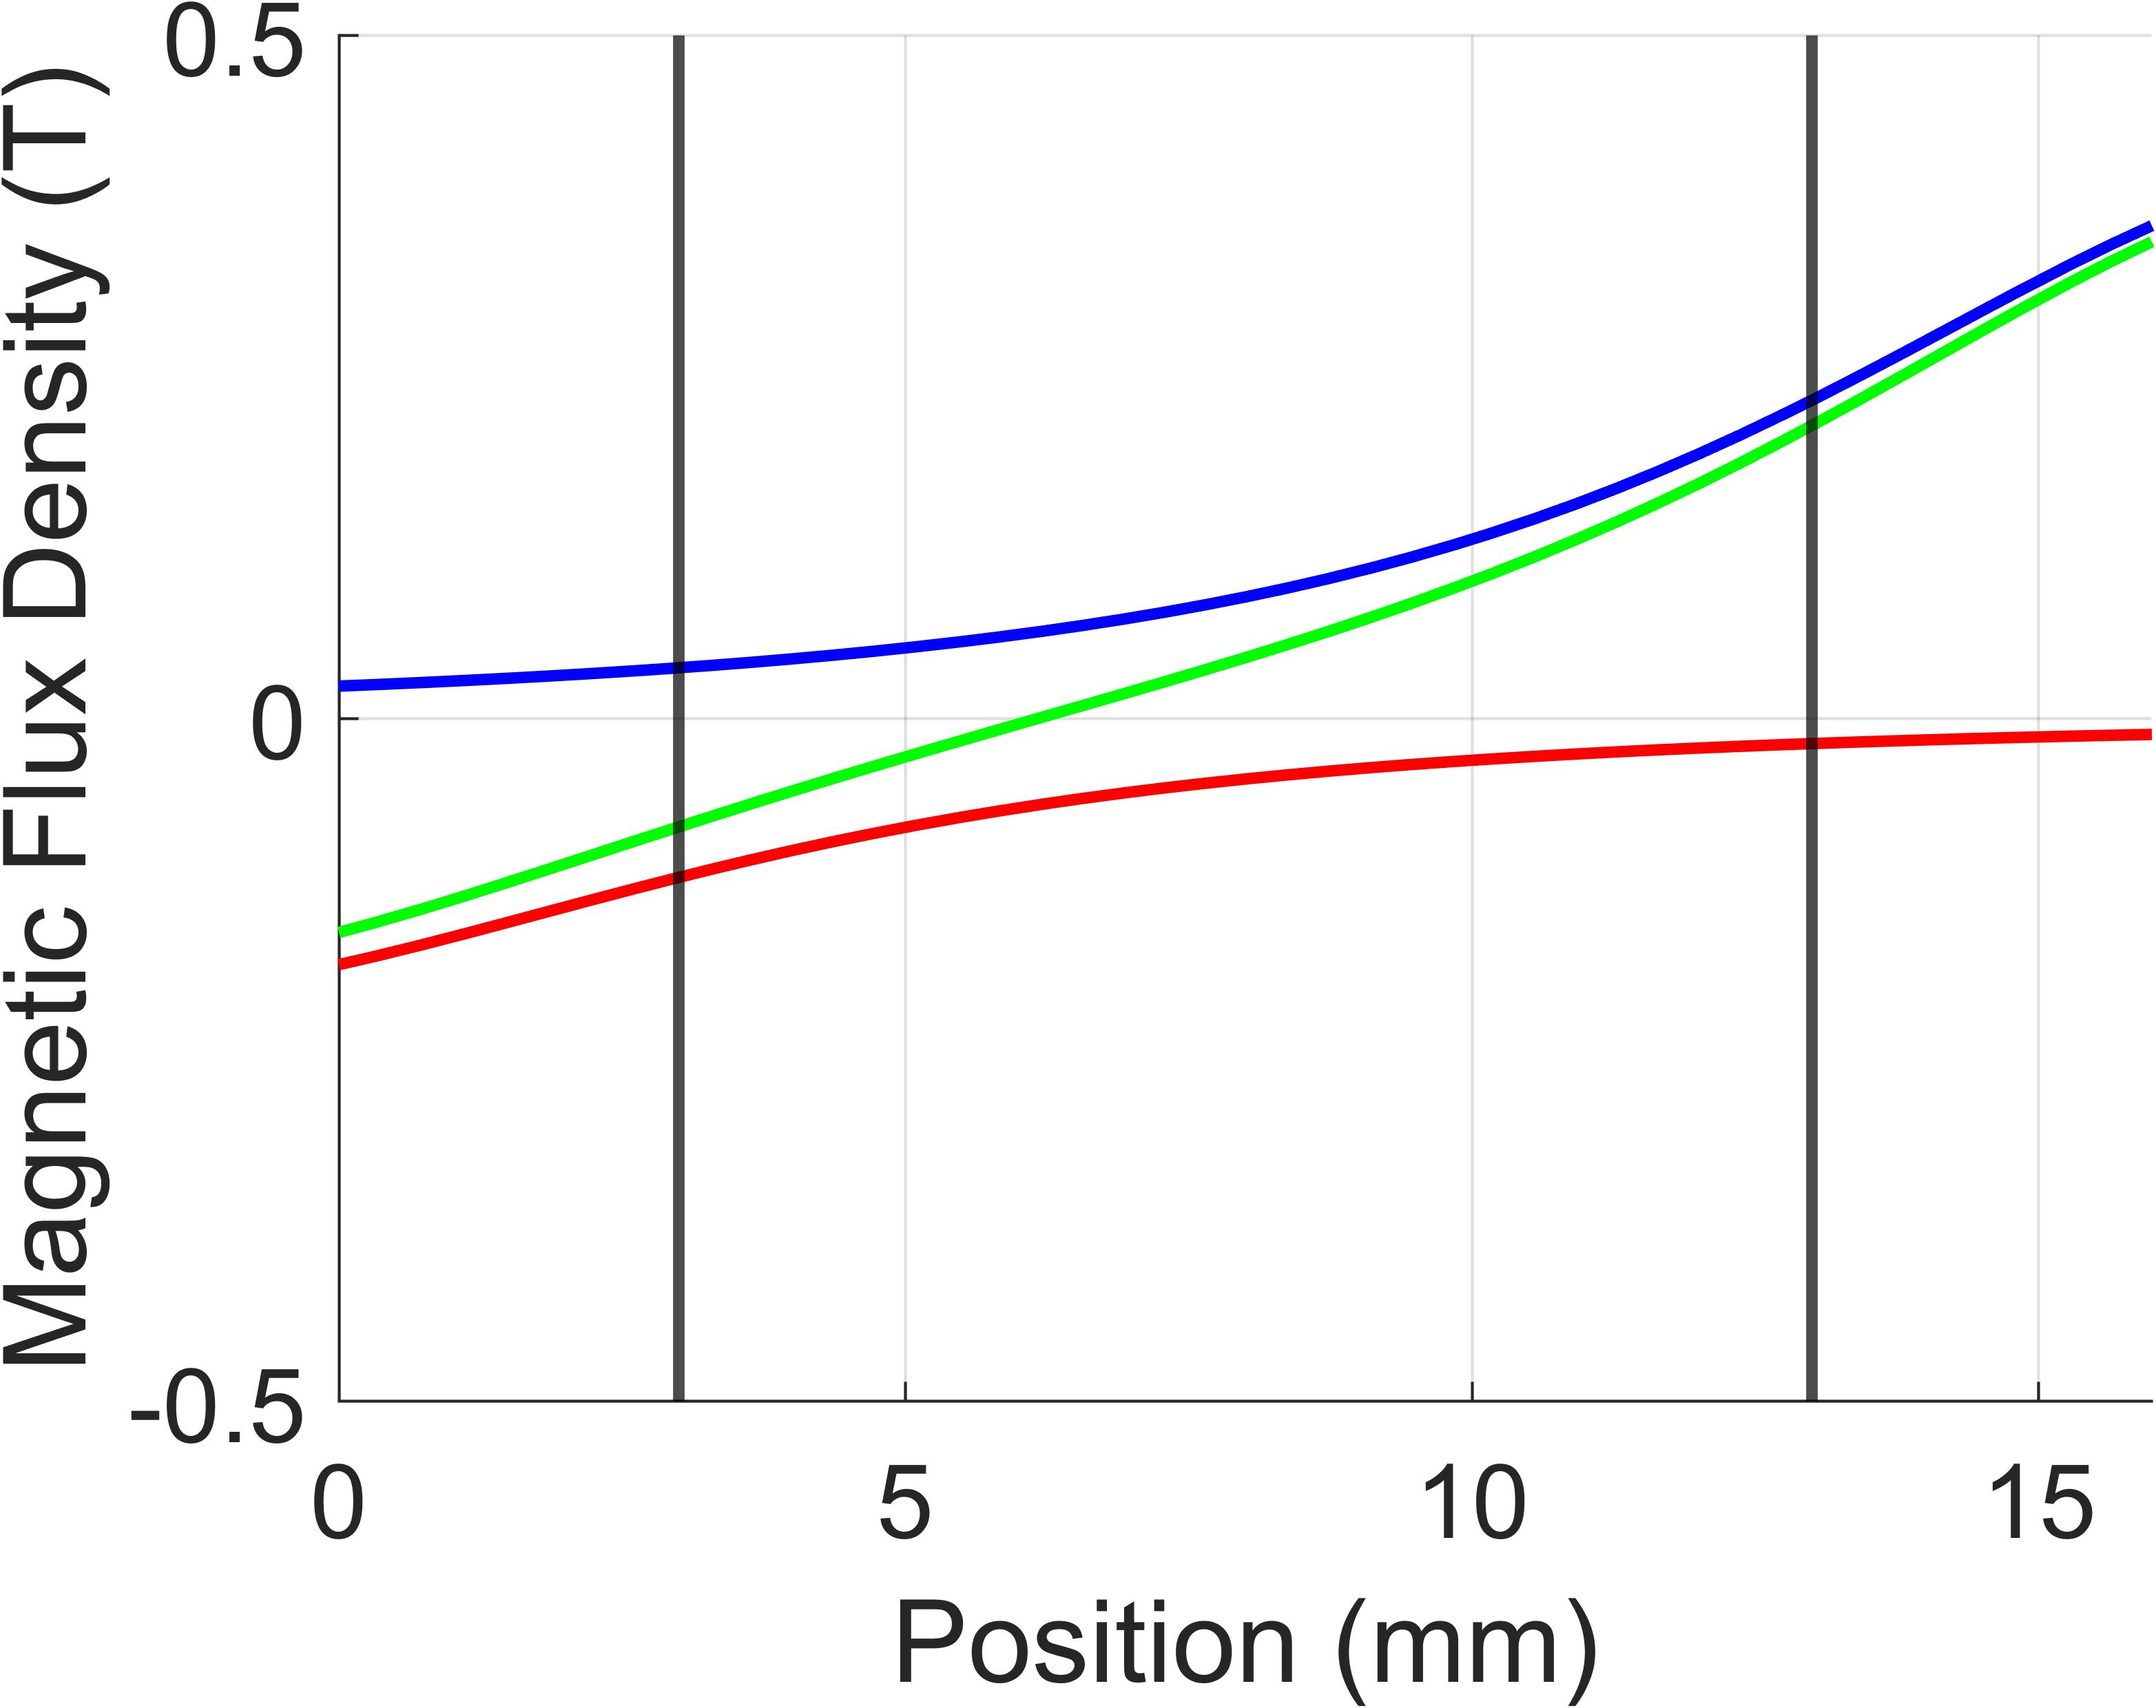
\includegraphics[width=.9\linewidth]{FluxOneTwentyDeg.jpg}
		\caption{\SI{120}{\degree} Phase}
		\label{fig:Flux120}
	\end{subfigure}
	\hfill
	\begin{subfigure}[b]{.475\textwidth}
		\centering
		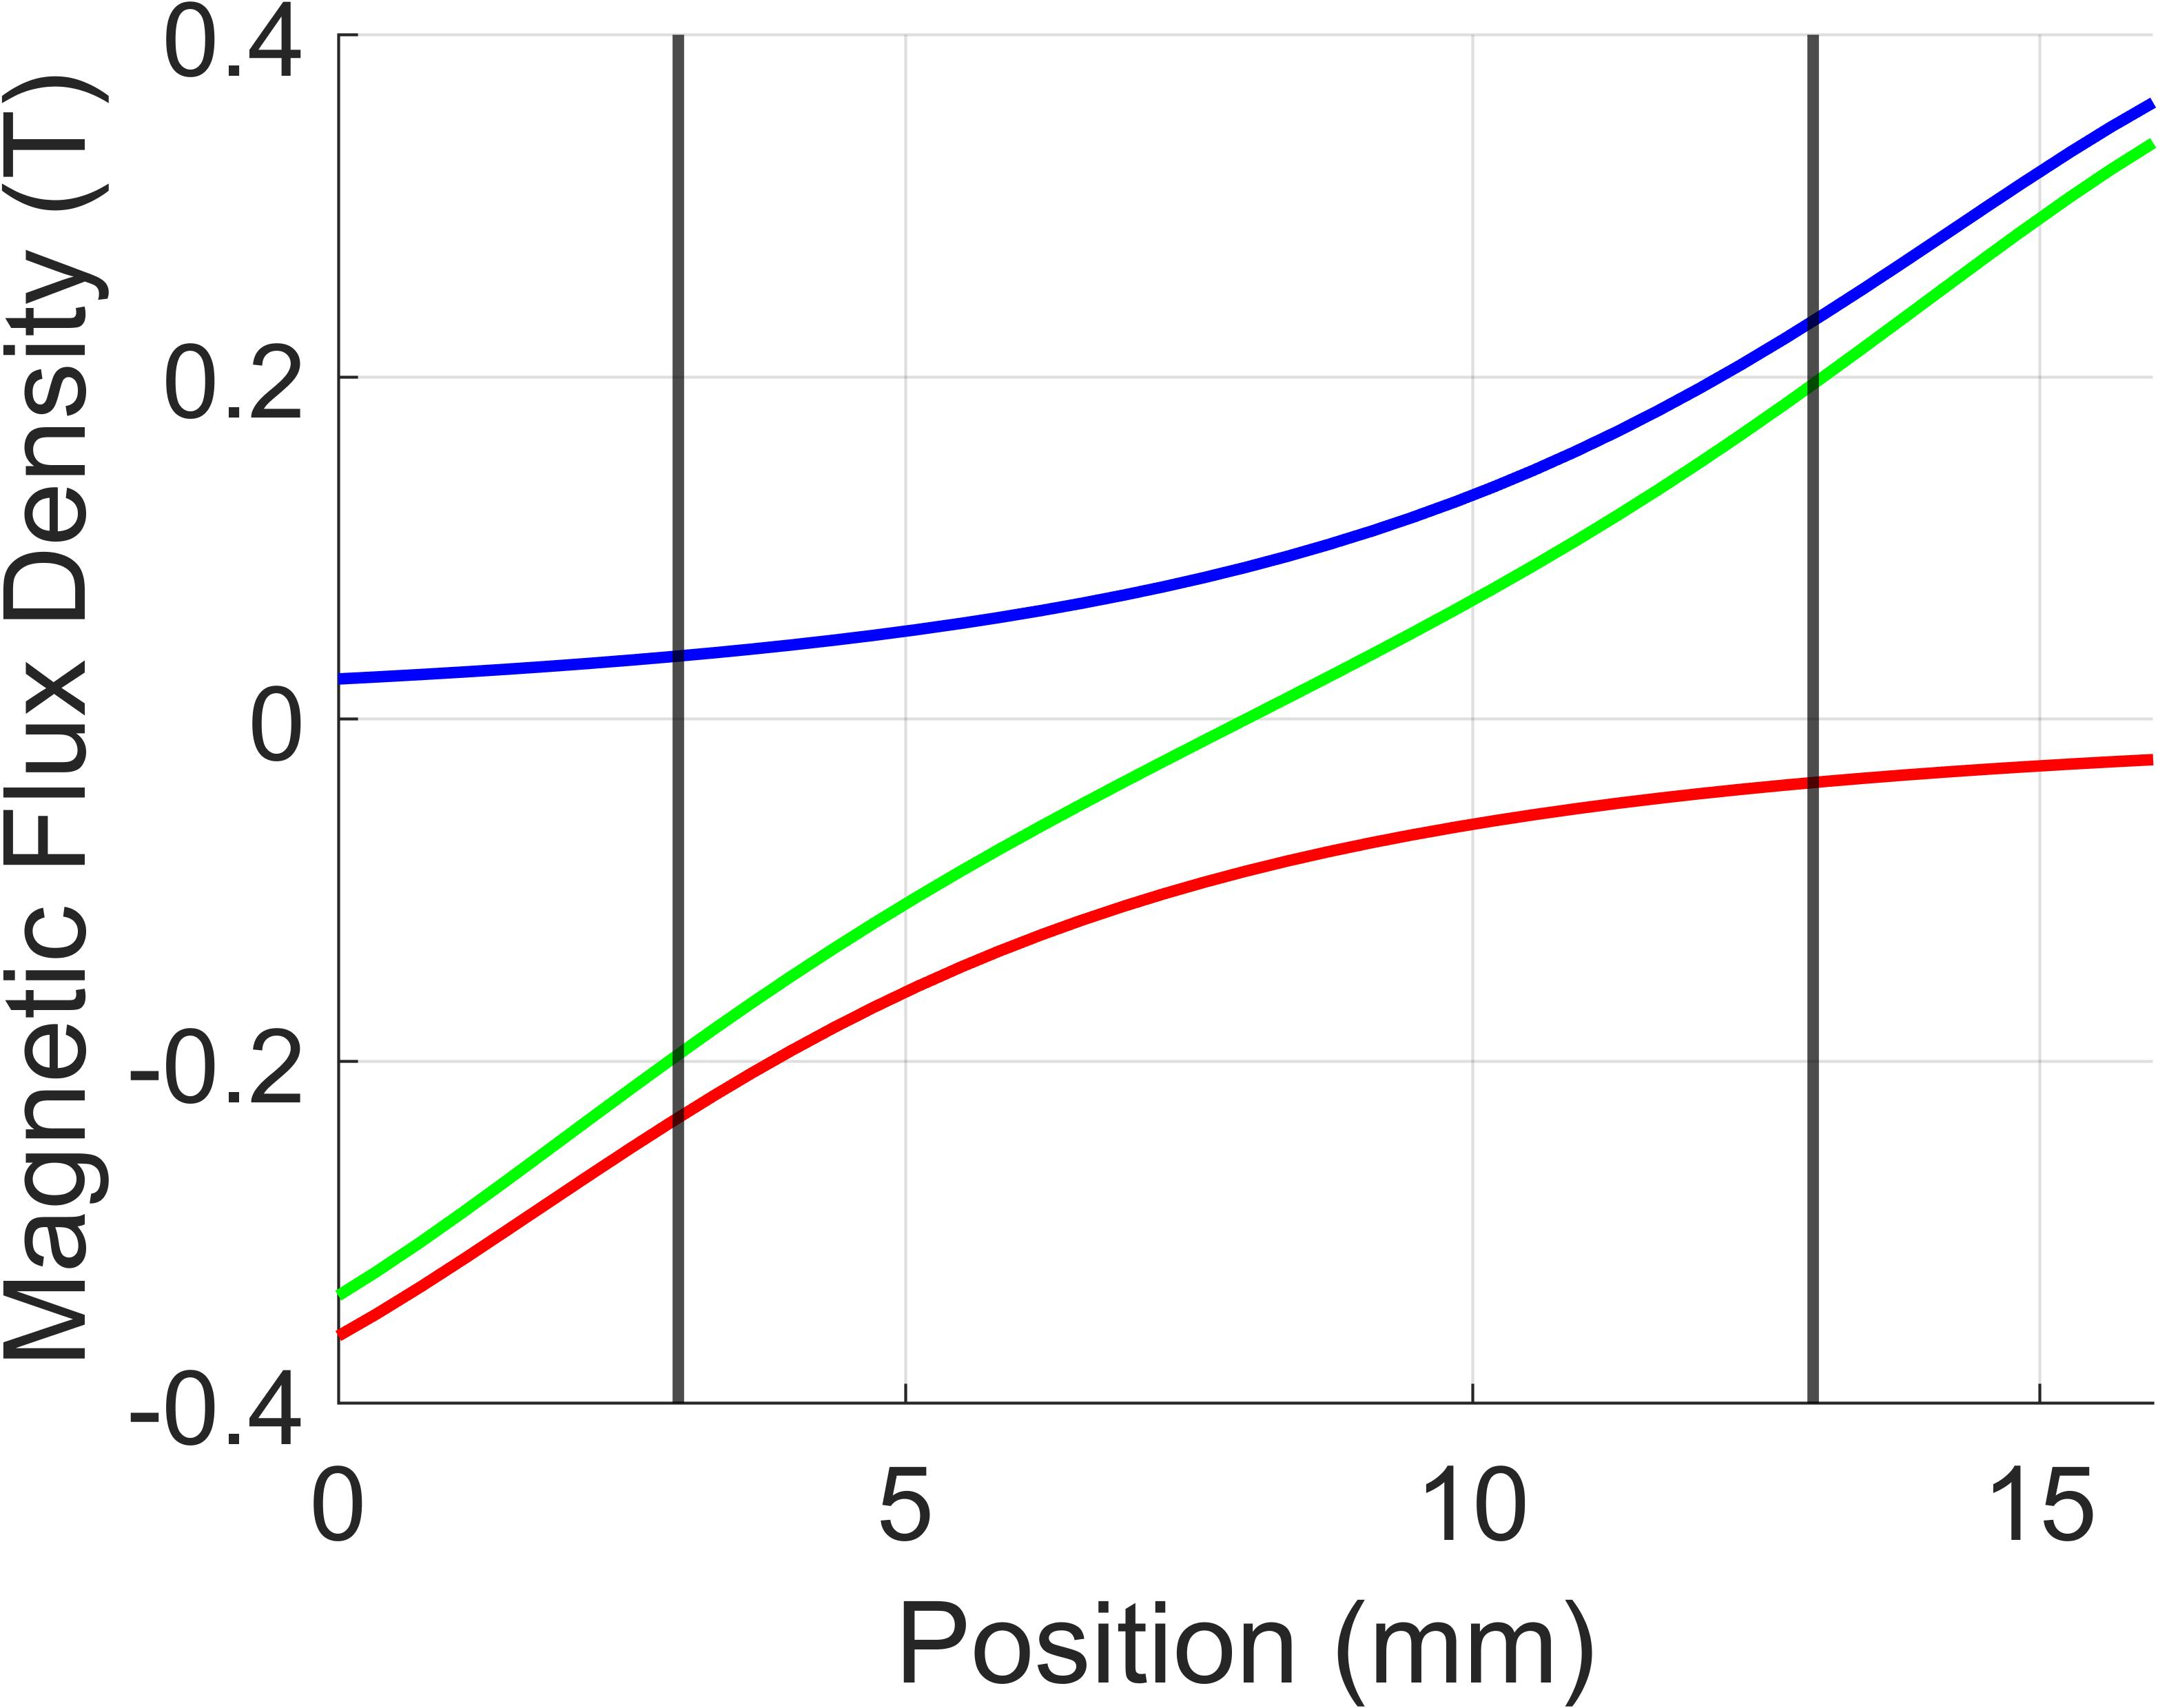
\includegraphics[width=.9\linewidth]{FluxOneEightyDeg.jpg}
		\caption{\SI{180}{\degree} Phase}
		\label{fig:Flux180}
	\end{subfigure}
	\begin{subfigure}{.475\textwidth}
	\centering
	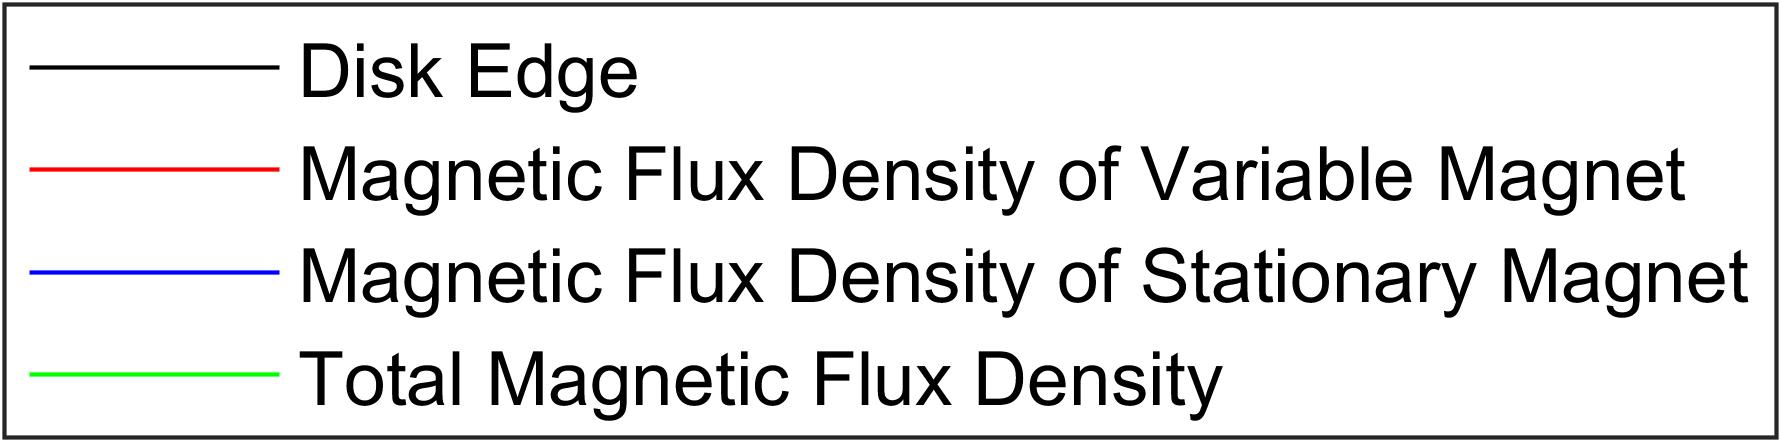
\includegraphics[width=\linewidth]{FluxLegend.jpg}
	\end{subfigure}
	\caption{Flux Distribution}
	\label{fig:Flux}
\end{figure}

\begin{figure}[H]
	\begin{center}
		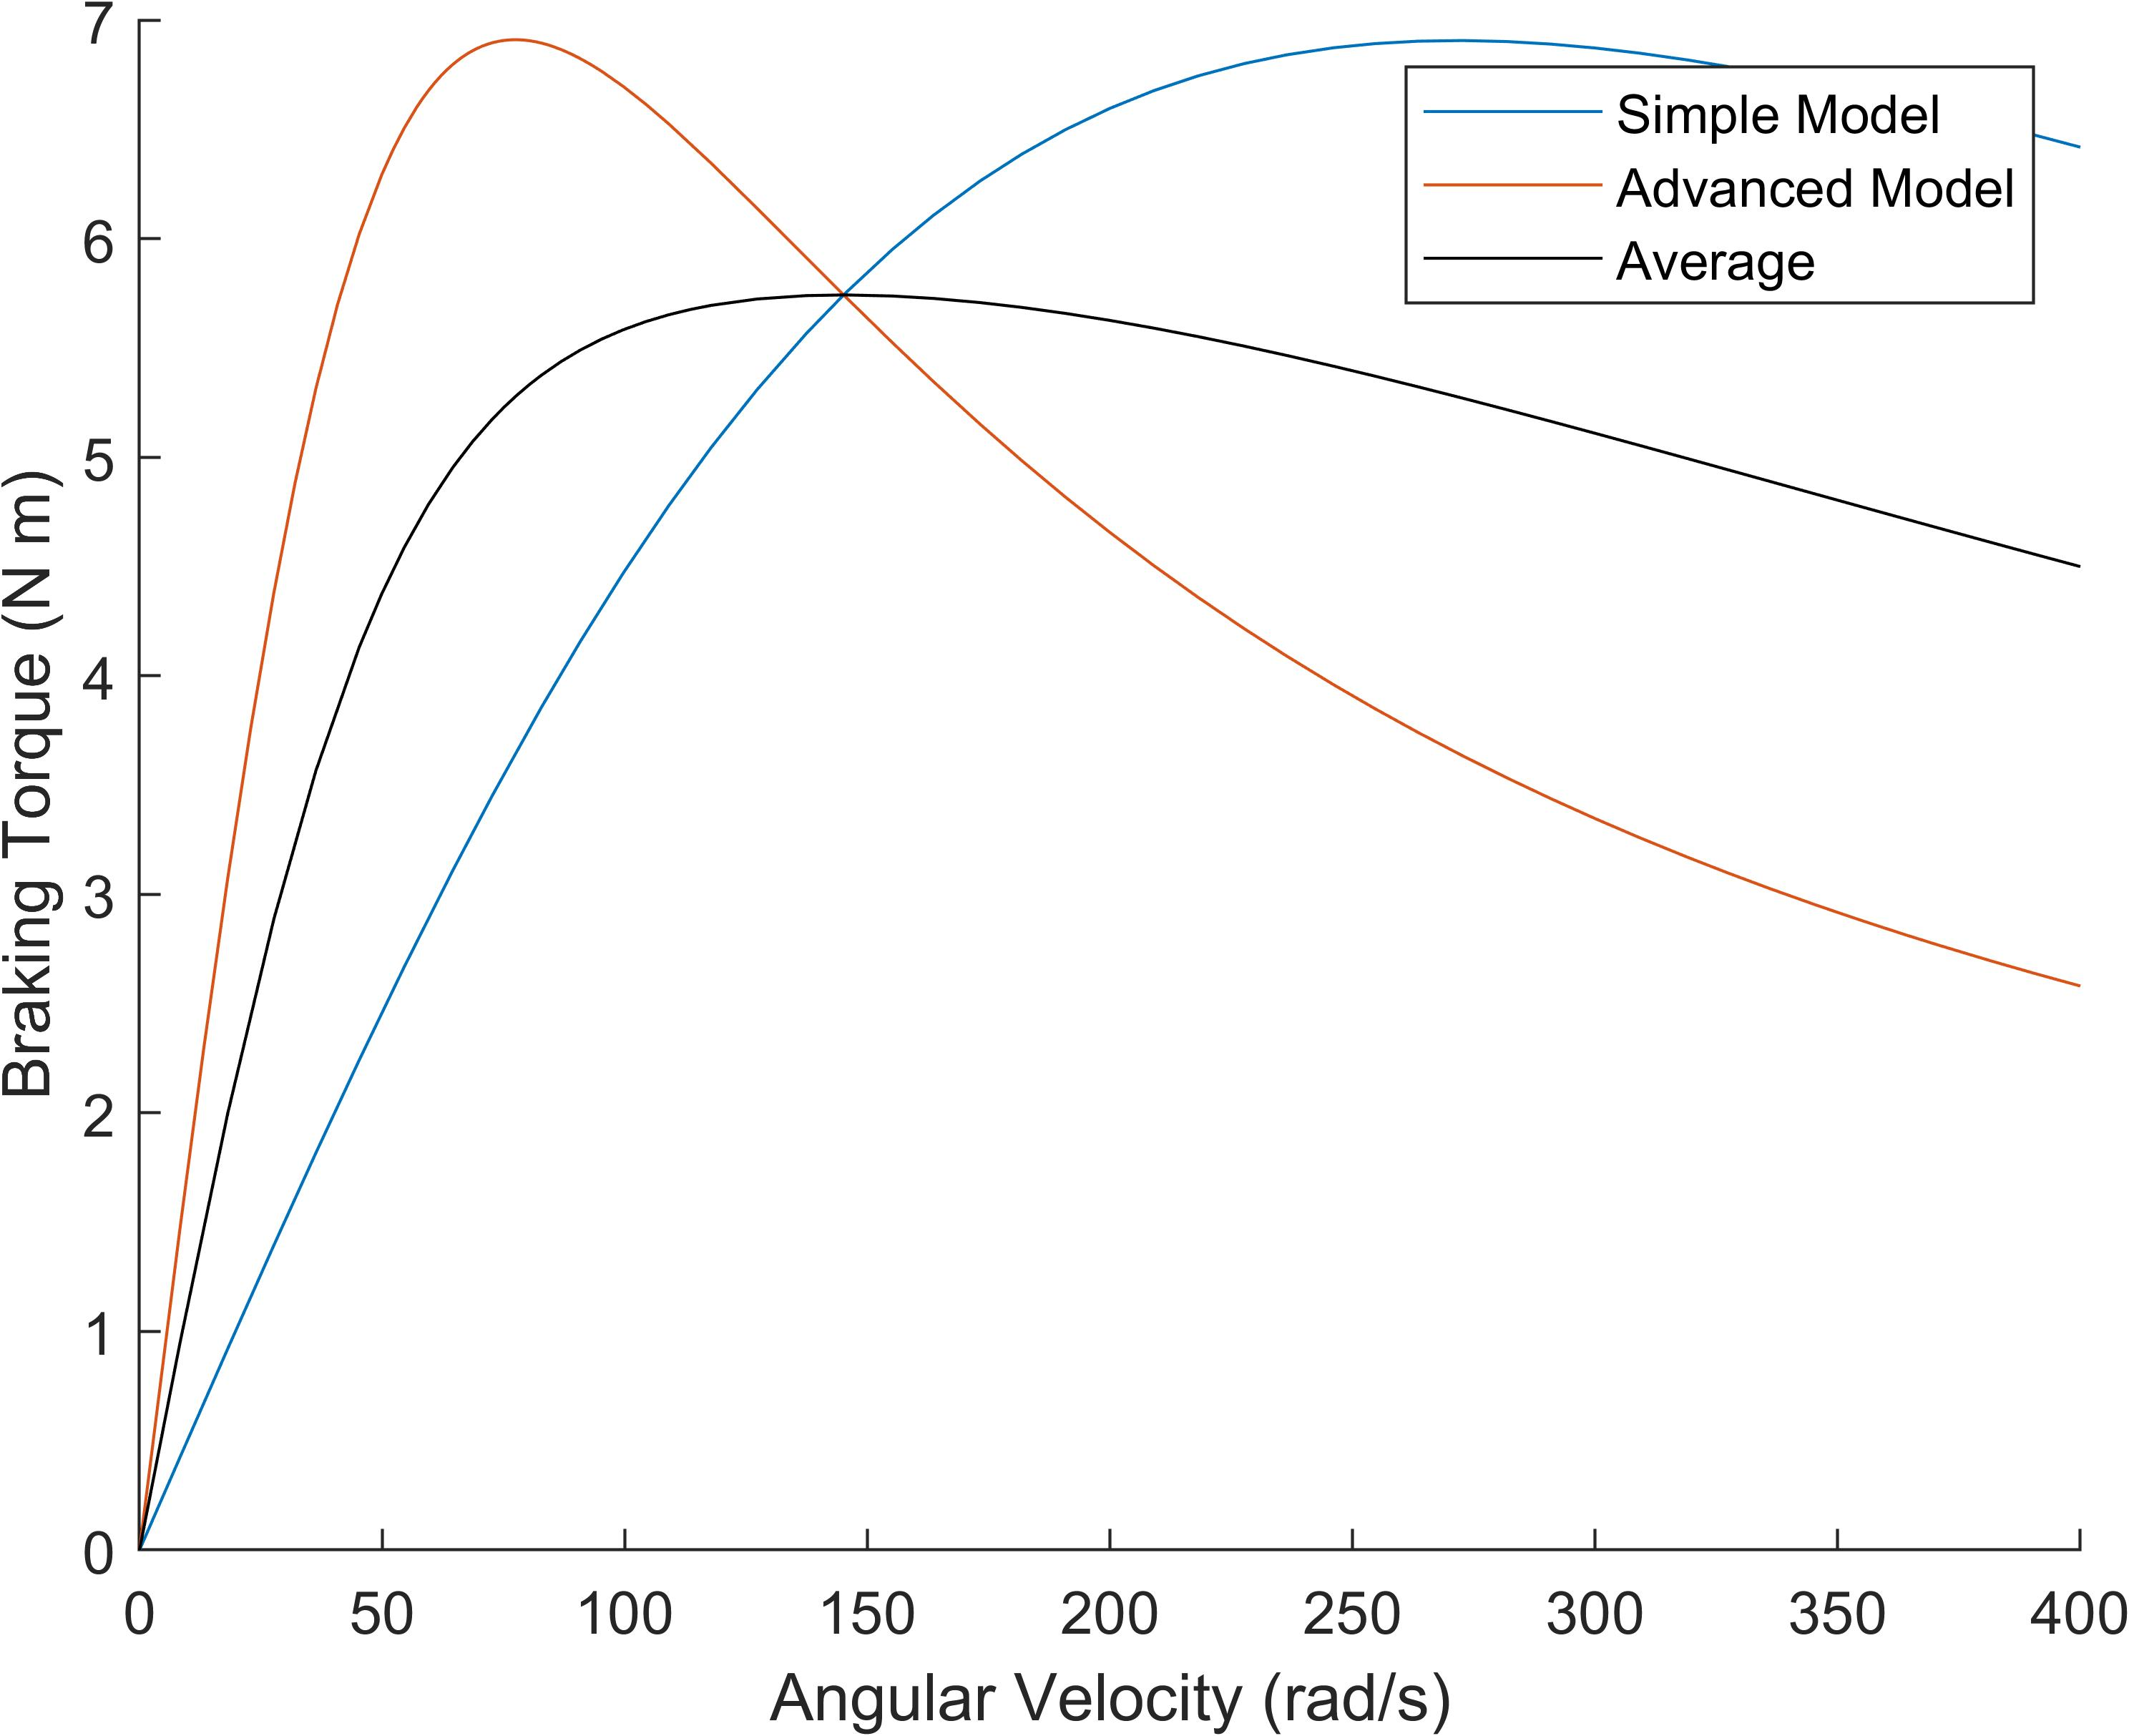
\includegraphics[width=0.8\textwidth]{Fig7.jpg}
		\caption{Figure 7}
		\label{fig:7}
	\end{center}
\end{figure}
\begin{figure}[H]
	\begin{center}
		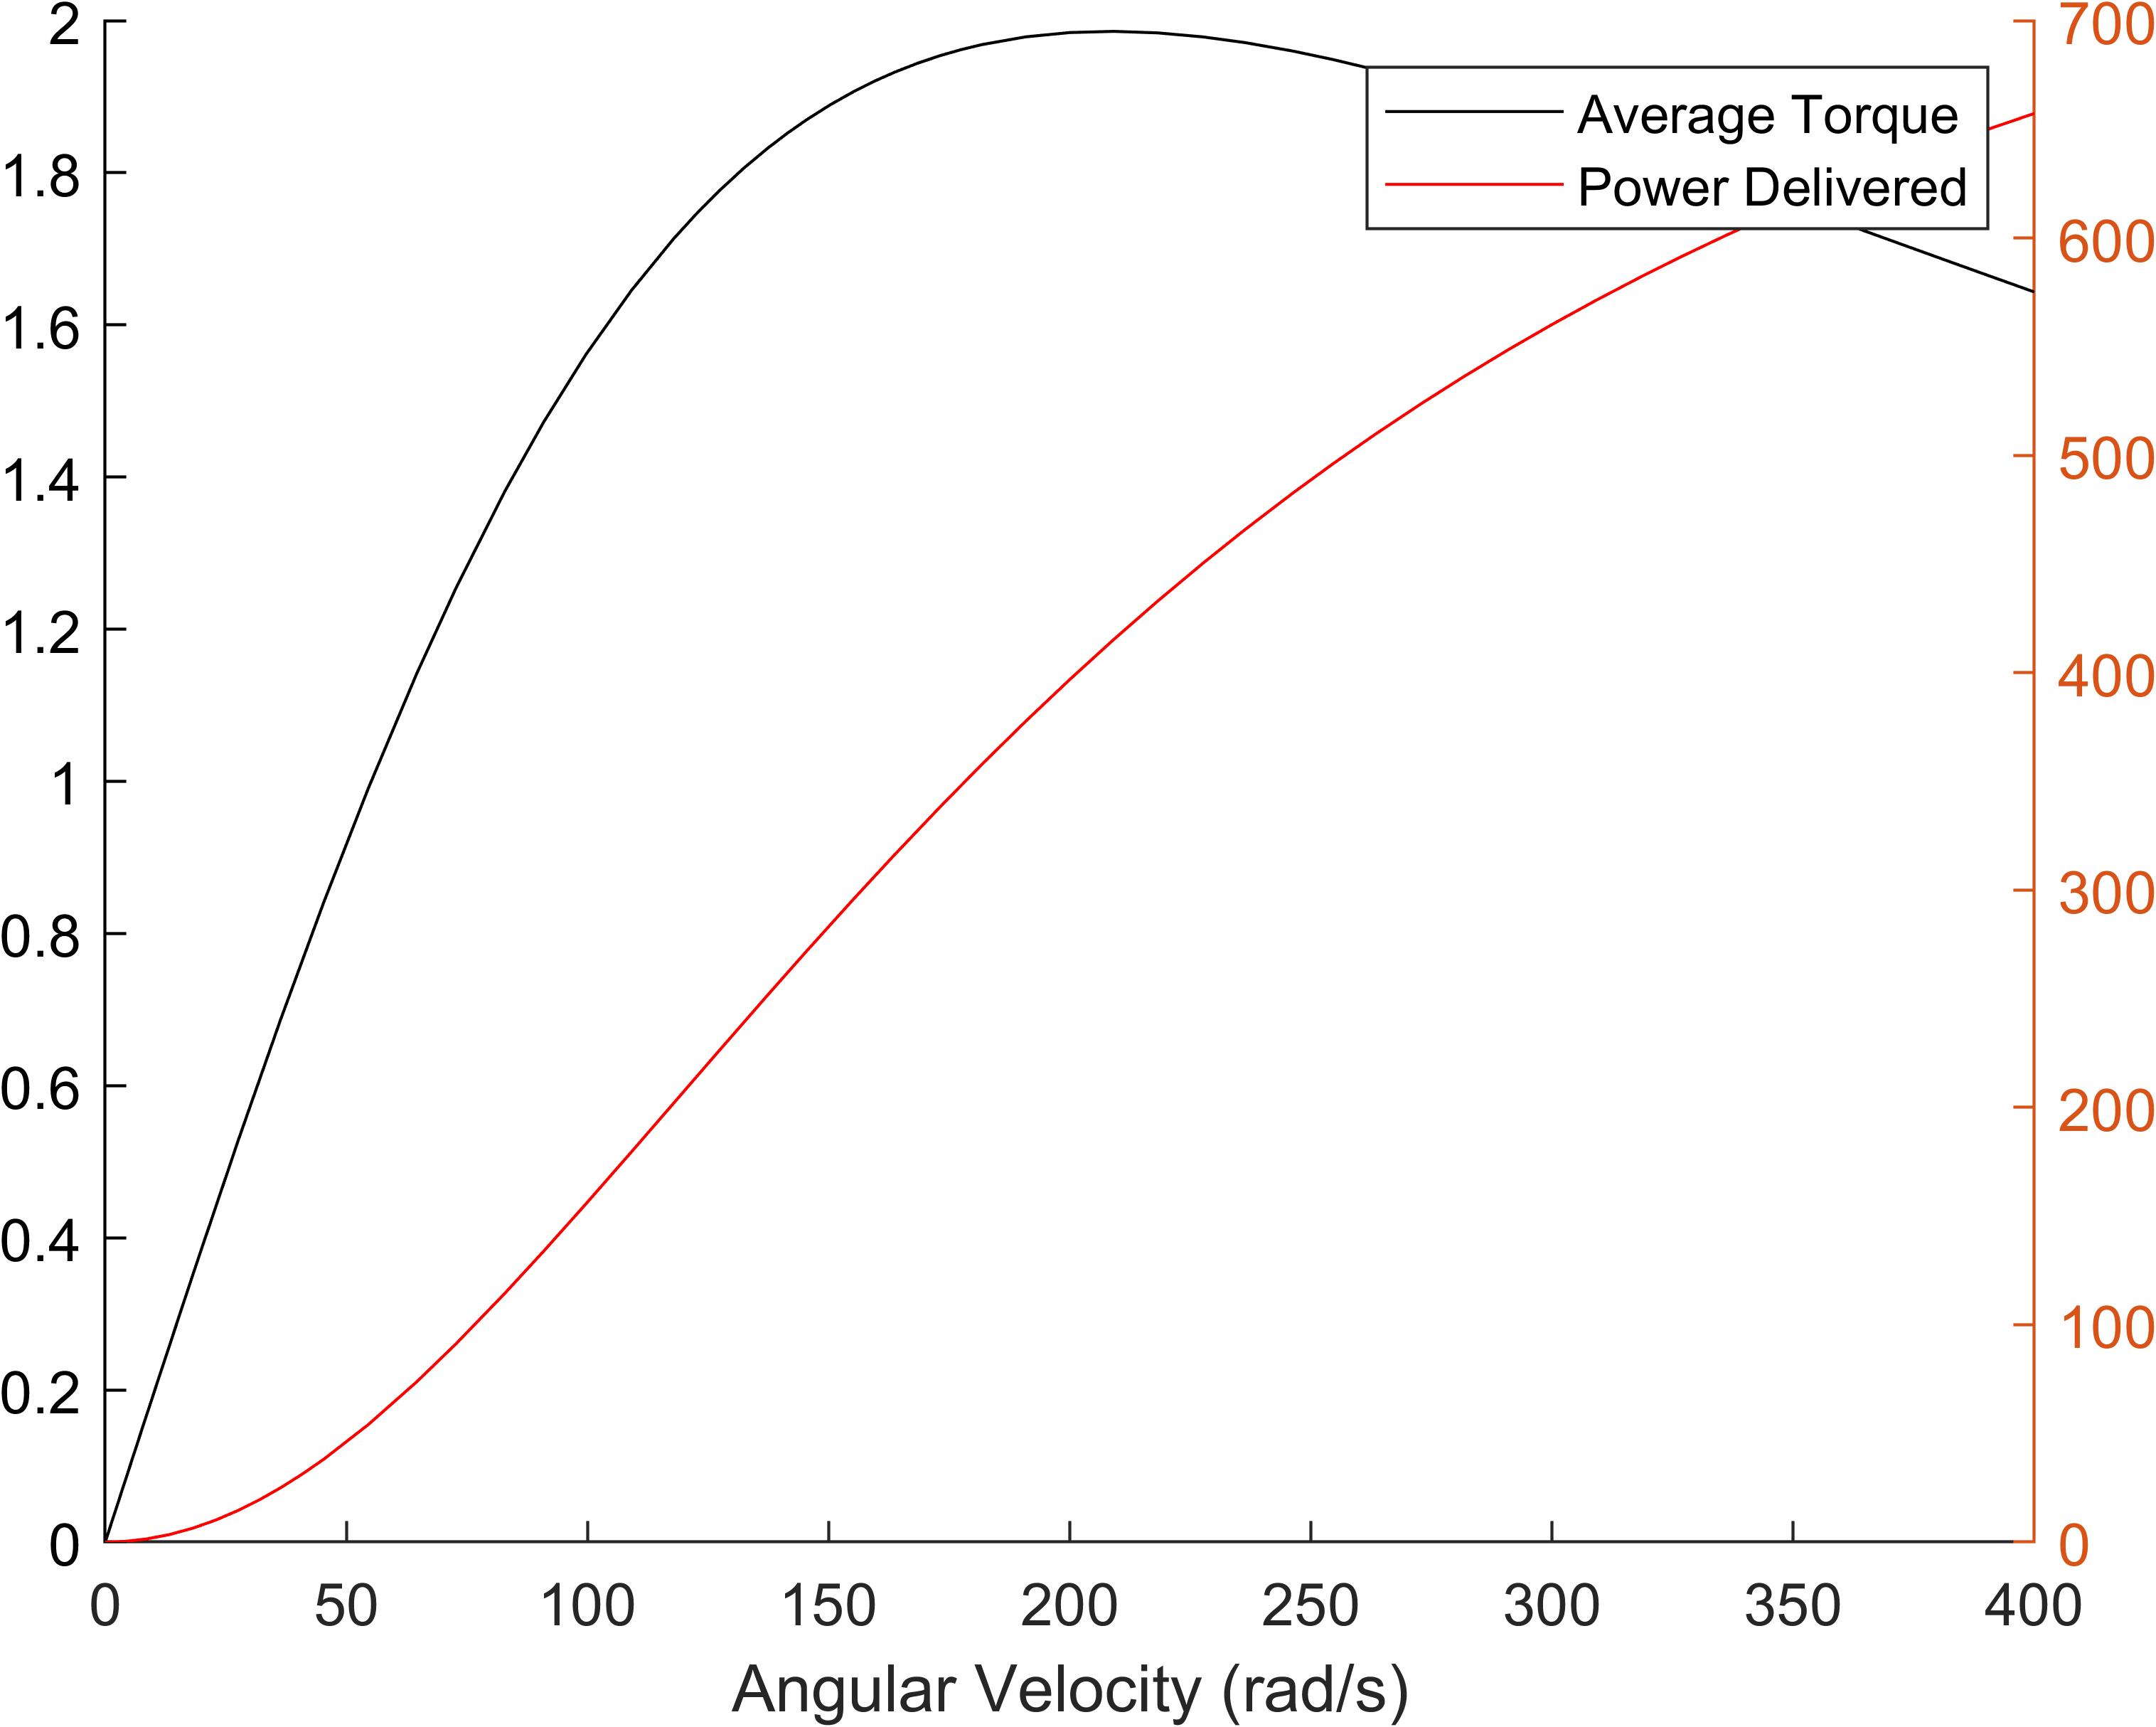
\includegraphics[width=0.8\textwidth]{Fig8.jpg}
		\caption{Figure 8}
		\label{fig:8}
	\end{center}
\end{figure}

\newpage
\section{Sensors}
Speed sensors are required to measure the speed of the cyclist ...
\subsection{Concept Evaluation}
Sensors are required to measure the angular velocity of both the rear cylinders. It was decided that using a infrared transmitter-receiver device with a reflective strip on the cylinder would be sufficient. The expected maximum sampling rate, as determined in section 